%%%%%%%%%%%%%%%%%%%%%%%%%%%%%%%%%%%%%%%%%
% a0poster Portrait Poster
% LaTeX Template
% Version 1.0 (22/06/13)
%
% The a0poster class was created by:
% Gerlinde Kettl and Matthias Weiser (tex@kettl.de)
% 
% This template has been downloaded from:
% http://www.LaTeXTemplates.com
%
% License:
% CC BY-NC-SA 3.0 (http://creativecommons.org/licenses/by-nc-sa/3.0/)
%
%%%%%%%%%%%%%%%%%%%%%%%%%%%%%%%%%%%%%%%%%

%-----------------------------------------------------------------------------
%	PACKAGES AND OTHER DOCUMENT CONFIGURATIONS
%-----------------------------------------------------------------------------

\documentclass[a0,portrait]{a0poster}

%% % sans-serif config:


\usepackage[english]{babel}
\usepackage[utf8]{inputenc}
\usepackage[T1]{fontenc}
\renewcommand{\familydefault}{\sfdefault}

\usepackage{multicol} % This is so we can have multiple columns of
                      % text side-by-side
\columnsep=100pt % This is the amount of white space between the
                 % columns in the poster
\columnseprule=3pt % This is the thickness of the black line between
                   % the columns in the poster

\usepackage[svgnames]{xcolor} % Specify colors by their 'svgnames',
                              % for a full list of all colors
                              % available see here:
                              % http://www.latextemplates.com/svgnames-colors

\usepackage{tgheros}


%% \usepackage{times} % Use the times font
%% \usepackage{palatino} % Uncomment to use the Palatino fon

\usepackage{graphicx} % Required for including images
\graphicspath{{figures/}} % Location of the graphics files
\usepackage{booktabs} % Top and bottom rules for table
\usepackage[font=small,labelfont=bf]{caption} % Required for
                                              % specifying captions to
                                              % tables and figures
\usepackage{amsfonts, amsmath, amsthm, amssymb} % For math fonts,
                                                % symbols and
                                                % environments
\usepackage{wrapfig} % Allows wrapping text around tables and figures

%\usepackage{sfmath}
\usepackage{sansmath} %additional math
\sansmath

\usepackage{mathsetup}

\usepackage{bibconfig}


\makeatletter
\g@addto@macro\normalsize{%
  \setlength\abovedisplayskip{18pt}
  \setlength\belowdisplayskip{18pt}
  \setlength\abovedisplayshortskip{16pt}
  \setlength\belowdisplayshortskip{16pt}
}
\makeatother


\addtolength{\parskip}{0.5\baselineskip}
\parindent 0pt

\definecolor{gblue}{RGB}{27,98,183}

\begin{document}

%-----------------------------------------------------------------------------
%	POSTER HEADER 
%-----------------------------------------------------------------------------

% The header is divided into two boxes:
% The first is 75% wide and houses the title, subtitle, names, university/organization and contact information
% The second is 25% wide and houses a logo for your university/organization or a photo of you
% The widths of these boxes can be easily edited to accommodate your content as you see fit
\vspace{-5cm}

%\fbox{
\begin{minipage}[b]{0.75\linewidth}
  \veryHuge \textbf{Non-random connectivity comes in pairs} \color{Black}\\[1.5cm] 
%\Huge\textit{}\\[2cm] % Subtitle
  \huge \textbf{Felix Z. Hoffmann$^{1,2}$, Jochen Triesch$^1$}\\[0.5cm] % Author(s)
\large $\quad ^1$Frankfurt Institute for Advanced Studies (FIAS), Johann Wolfgang Goethe University, Frankfurt am Main, Germany\\[0.2cm] % University/organization
$\quad ^2$International Max Planck Research School for Neural Circuits, Max Planck Institute for Brain Research, Frankfurt am Main, Germany\\[0.4cm]
\Large \texttt{hoffmann@fias.uni-frankfurt.de}\\
\end{minipage}
%}
%
%\fbox{
\begin{minipage}[b]{0.25\linewidth}
  \centering
  
  
\includegraphics[width=10cm]{goethe-logo.pdf}\\
  \vspace{2.8cm}
  
\includegraphics[width=12.5cm]{FIAS-logo.pdf}\\
  \vspace{2cm}
  
\end{minipage}
%}
%\vspace{0.2cm} % A bit of extra whitespace between the header and poster content

%-----------------------------------------------------------------------------

\begin{multicols}{2} % This is how many columns your poster will be broken into, a portrait poster is generally split into 2 columns

  
\begin{abstract}
  \medskip
  
  Overrepresentation of bidirectional connections in local cortical networks has been repeatedly reported and is in the focus of the ongoing discussion of non-random connectivity.
  %
  Here we show in a brief mathematical analysis that in a network in which connection probabilities are symmetric in pairs, $P_{ij} = P_{ji}$, the occurrence of bidirectional connections and non-random structures are inherently linked; an overabundance of reciprocally connected pairs emerges necessarily when the network structure deviates from a random network in any form.
  %
  %For two distributions of connection probabilities, the discrete two-point distribution and continuous gamma distribution, we quantify how a more organized structure increases reciprocity in the network.

\end{abstract}
  
  \section*{Introduction}

Increasing evidence implies that \textbf{cortical microcircuitry is highly structured} \cite{Song2005,Perin2011}.
%
The relative occurrence of bidirectionally connected pairs has been of particular interest: 

  
\section*{Results}

\textit{Define a random network model in which node-to-node connection probabilities themselves follow a random distribution; some pairs of neurons have a higher chance to be connected than others.}


Consider a random network model of $N$ neurons in which a connection from node $i$ to node $j$ exists with probability $P_{ij}$.
%
Here, the $P_{ij}$, with $i,j = 1,\dots,N$ and $i \neq j$, are identically distributed random variables in $[0,1]$, yielding a probability of connection for each ordered pair of nodes in the network.


\textit{Next, calculate the overrepresentation of bidirectional connection as we would measure in an experiment.}

The overall connection probability $\mu$, that is the chance to have a connection from a random node $i$ to another node $j$, is
\begin{align}
\mu = \E(P_{ij}).
\end{align}
For example, if the $P_{ij}$ have a probability density function $f$ with essential support in $[0,1]$, we can compute the connection fraction as
\begin{align}
  \mu = \int_0^1 x f(x)\,dx.
\end{align}
The probability for random pair of nodes $i$ and $j$ to be connected reciprocally is then
\begin{align}
P_{\mathrm{rec}} = \E(P_{ij} P_{ji}).
\end{align}




  \vspace{8cm}
  
  
\section*{Two-point distribution}

Consider $P_{ij}$ to follow the discrete \textbf{two-point distribution}, where
\begin{align}
  \Prob(P_{ij}=x)=p \quad \mathrm{and} \quad \Prob(P_{ij}=y)=1-p.
\end{align}

We derive an expression for the relative occurrence of reciprocal pairs $\varrho$ as
\begin{align}
\varrho = \frac{x+y}{\mu} - \frac{xy}{\mu^2}.
\end{align}

\begin{center}\vspace{1cm}
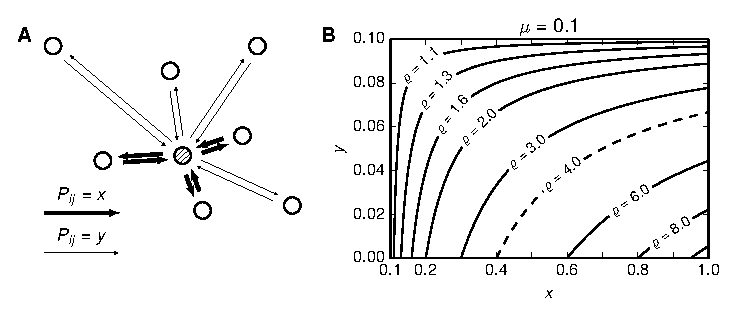
\includegraphics[width=0.9\linewidth]{two_point_full_figure.pdf}
\captionof{figure}{\textbf{A} Sketch of a network with connection probabilities $x$ and $y$ \textbf{B} For $\mu=0.1$ fixed, different pairings of $x$ and $y$ can induce high values of the relative occurrence of bidirectionally connected pairs $\varrho$. Dashed line marks an overrepresentation of $\varrho=4$ as observed for layer 5 pyramidal neurons in the rat visual cortex \cite{Song2005}.}
\end{center}\vspace{1cm}




  
\section*{Truncated gamma distribution}

Consider the $P_{ij}$ to follow the continuous \textbf{truncated gamma distribution}, which is given by the density function $f^T$ as
\begin{align}
  f_{\alpha,\beta}^T(x) = \begin{cases} K_{\alpha, \beta}\,
\frac{1}{\beta^{\alpha}\Gamma(\alpha)}\, x^{\alpha-1}\,e^{-x/\beta} & 0 \leq x \leq 1 \\
0 & \text{otherwise},
\end{cases}
\end{align}

where the normalization factor $K_{\alpha,\beta}$ is the inverse of the cumulative
probability that $x \leq 1$ of the untruncated gamma distribution 
\begin{align}
  K_{\alpha,\beta} = \left(\int_0^{1} \frac{1}{\beta^{\alpha}\Gamma(\alpha)}\, x^{\alpha-1}\,e^{-x/\beta} \, dx \right)^{-1}.
\end{align}
When the overall connection probability $\mu$ is fixed, only one free parameter remains, and the relative overrepresentation of bidirectional connections $\varrho$ can be approximated as
\begin{align}
 \varrho \approx  1 + \frac{1}{\alpha}.
\end{align}

\begin{center}\vspace{1cm}
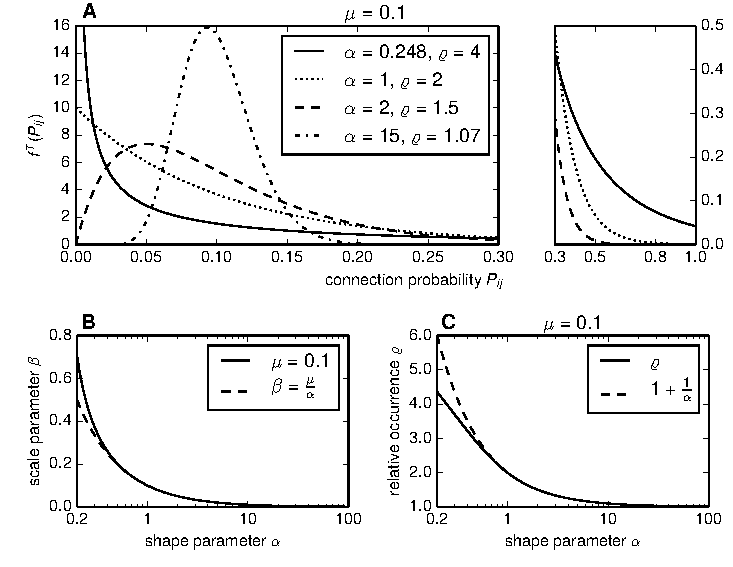
\includegraphics[width=0.9\linewidth]{gamma_figure.pdf}
\captionof{figure}{ \textbf{A} Probability density functions of the
  truncated gamma distribution for different shape parameters $\alpha$
  and the induced relative overrepresentation $\varrho$ in the network
  with such distributed connection probabilities $P_{ij}$. For a given
  $\alpha$, the scale parameter $\beta$ was chosen such that $\mu =
  0.1$. \textbf{B} Contour of $\alpha$, $\beta$ pairings
  that yield an overall connection probability of $\mu =
  0.1$. \textbf{C} Relative occurrence $\varrho$ in dependence on
  $\alpha$ for fixed $\mu = 0.1$. For $\alpha \geq 1$ this
  relationship is well approximated by $\varrho \approx 1 +
  \frac{1}{\alpha}$.}
\end{center}\vspace{1cm}

  \section*{Conclusions}

\begin{itemize}
\item Pellentesque eget orci eros. Fusce ultricies, tellus et pellentesque fringilla, ante massa luctus libero, quis tristique purus urna nec nibh. Phasellus fermentum rutrum elementum. Nam quis justo lectus.
\item Vestibulum sem ante, hendrerit a gravida ac, blandit quis magna.
\item Donec sem metus, facilisis at condimentum eget, vehicula ut massa. Morbi consequat, diam sed convallis tincidunt, arcu nunc.
\item Nunc at convallis urna. isus ante. Pellentesque condimentum dui. Etiam sagittis purus non tellus tempor volutpat. Donec et dui non massa tristique adipiscing.
\end{itemize}


  %%-----------------------------------------------------------------------------
%	ABSTRACT
%-----------------------------------------------------------------------------

\begin{abstract}

Sed fringilla tempus hendrerit. Vestibulum ante ipsum primis in faucibus orci luctus et ultrices posuere cubilia Curae; Etiam ut elit sit amet metus lobortis consequat sit amet in libero. Lorem ipsum dolor sit amet, consectetur adipiscing elit. Phasellus vel sem magna. Nunc at convallis urna. isus ante. Pellentesque condimentum dui. Etiam sagittis purus non tellus tempor volutpat. Donec et dui non massa tristique adipiscing. Quisque vestibulum eros eu. Phasellus imperdiet, tortor vitae congue bibendum, felis enim sagittis lorem, et volutpat ante orci sagittis mi. Morbi rutrum laoreet semper. Morbi accumsan enim nec tortor consectetur non commodo nisi sollicitudin. Proin sollicitudin. Pellentesque eget orci eros. Fusce ultricies, tellus et pellentesque fringilla, ante massa luctus libero, quis tristique purus urna nec nibh.

\end{abstract}

%-----------------------------------------------------------------------------
%	INTRODUCTION
%-----------------------------------------------------------------------------

\section*{Introduction}

Aliquam non lacus dolor, \textit{a aliquam quam} \cite{Smith:2012qr}. Cum sociis natoque penatibus et magnis dis parturient montes, nascetur ridiculus mus. Nulla in nibh mauris. Donec vel ligula nisi, a lacinia arcu. Sed mi dui, malesuada vel consectetur et, egestas porta nisi. Sed eleifend pharetra dolor, et dapibus est vulputate eu. \textbf{Integer faucibus elementum felis vitae fringilla.} In hac habitasse platea dictumst. Duis tristique rutrum nisl, nec vulputate elit porta ut. Donec sodales sollicitudin turpis sed convallis. Etiam mauris ligula, blandit adipiscing condimentum eu, dapibus pellentesque risus.

\textit{Aliquam auctor}, metus id ultrices porta, risus enim cursus sapien, quis iaculis sapien tortor sed odio. Mauris ante orci, euismod vitae tincidunt eu, porta ut neque. Aenean sapien est, viverra vel lacinia nec, venenatis eu nulla. Maecenas ut nunc nibh, et tempus libero. Aenean vitae risus ante. Pellentesque condimentum dui. Etiam sagittis purus non tellus tempor volutpat. Donec et dui non massa tristique adipiscing.

%-----------------------------------------------------------------------------
%	OBJECTIVES
%-----------------------------------------------------------------------------

\section*{Main Objectives}

\begin{enumerate}
\item Lorem ipsum dolor sit amet, consectetur.
\item Nullam at mi nisl. Vestibulum est purus, ultricies cursus volutpat sit amet, vestibulum eu.
\item Praesent tortor libero, vulputate quis elementum a, iaculis.
\item Phasellus a quam mauris, non varius mauris. Fusce tristique, enim tempor varius porta, elit purus commodo velit, pretium mattis ligula nisl nec ante.
\item Ut adipiscing accumsan sapien, sit amet pretium.
\item Estibulum est purus, ultricies cursus volutpat
\item Nullam at mi nisl. Vestibulum est purus, ultricies cursus volutpat sit amet, vestibulum eu.
\item Praesent tortor libero, vulputate quis elementum a, iaculis.
\end{enumerate}

%-----------------------------------------------------------------------------
%	MATERIALS AND METHODS
%-----------------------------------------------------------------------------

\section*{Materials and Methods}

Fusce magna risus, molestie ut porttitor in, consectetur sed mi. Vestibulum ante ipsum primis in faucibus orci luctus et ultrices posuere cubilia Curae; Pellentesque consectetur blandit pellentesque. Sed odio justo, viverra nec porttitor vel, lacinia a nunc. Suspendisse pulvinar euismod arcu, sit amet accumsan enim fermentum quis. In id mauris ut dui feugiat egestas. Vestibulum ac turpis lacinia nisl commodo sagittis eget sit amet sapien.

%------------------------------------------------

\subsection*{Mathematical Section}

Nulla vel nisl sed mauris auctor mollis non sed. 

\begin{equation}
E = mc^{2}
\label{eqn:Einstein}
\end{equation}

Curabitur mi sem, pulvinar quis aliquam rutrum. (1) edf (2)
, $\Omega=[-1,1]^3$, maecenas leo est, ornare at. $z=-1$ edf $z=1$ sed interdum felis dapibus sem. $x$ set $y$ ytruem. 
Turpis $j$ amet accumsan enim $y$-lacina; 
ref $k$-viverra nec porttitor $x$-lacina. 

Vestibulum ac diam a odio tempus congue. Vivamus id enim nisi:

\begin{eqnarray}
\cos\bar{\phi}_k Q_{j,k+1,t} + Q_{j,k+1,x}+\frac{\sin^2\bar{\phi}_k}{T\cos\bar{\phi}_k} Q_{j,k+1} &=&\nonumber\\ 
-\cos\phi_k Q_{j,k,t} + Q_{j,k,x}-\frac{\sin^2\phi_k}{T\cos\phi_k} Q_{j,k}\label{edgek}
\end{eqnarray}
and
\begin{eqnarray}
\cos\bar{\phi}_j Q_{j+1,k,t} + Q_{j+1,k,y}+\frac{\sin^2\bar{\phi}_j}{T\cos\bar{\phi}_j} Q_{j+1,k}&=&\nonumber \\
-\cos\phi_j Q_{j,k,t} + Q_{j,k,y}-\frac{\sin^2\phi_j}{T\cos\phi_j} Q_{j,k}.\label{edgej}
\end{eqnarray} 

Nulla sed arcu arcu. Duis et ante gravida orci venenatis tincidunt. Fusce vitae lacinia metus. Pellentesque habitant morbi. $\mathbf{A}\underline{\xi}=\underline{\beta}$ Vim $\underline{\xi}$ enum nidi $3(P+2)^{2}$ lacina. Id feugain $\mathbf{A}$ nun quis; magno.

%-----------------------------------------------------------------------------
%	RESULTS 
%-----------------------------------------------------------------------------

\section*{Results}

Donec faucibus purus at tortor egestas eu fermentum dolor facilisis. Maecenas tempor dui eu neque fringilla rutrum. Mauris \emph{lobortis} nisl accumsan. Aenean vitae risus ante.
%
\begin{wraptable}{l}{12cm} % Left or right alignment is specified in the first bracket, the width of the table is in the second
\begin{tabular}{l l l}
\toprule
\textbf{Treatments} & \textbf{Response 1} & \textbf{Response 2}\\
\midrule
Treatment 1 & 0.0003262 & 0.562 \\
Treatment 2 & 0.0015681 & 0.910 \\
Treatment 3 & 0.0009271 & 0.296 \\
\bottomrule
\end{tabular}
\captionof{table}{\color{Green} Table caption}
\end{wraptable}
%
Phasellus imperdiet, tortor vitae congue bibendum, felis enim sagittis lorem, et volutpat ante orci sagittis mi. Morbi rutrum laoreet semper. Morbi accumsan enim nec tortor consectetur non commodo nisi sollicitudin. Proin sollicitudin. Pellentesque eget orci eros. Fusce ultricies, tellus et pellentesque fringilla, ante massa luctus libero, quis tristique purus urna nec nibh.

Nulla ut porttitor enim. Suspendisse venenatis dui eget eros gravida tempor. Mauris feugiat elit et augue placerat ultrices. Morbi accumsan enim nec tortor consectetur non commodo. Pellentesque condimentum dui. Etiam sagittis purus non tellus tempor volutpat. Donec et dui non massa tristique adipiscing. Quisque vestibulum eros eu. Phasellus imperdiet, tortor vitae congue bibendum, felis enim sagittis lorem, et volutpat ante orci sagittis mi. Morbi rutrum laoreet semper. Morbi accumsan enim nec tortor consectetur non commodo nisi sollicitudin.

\begin{center}\vspace{1cm}
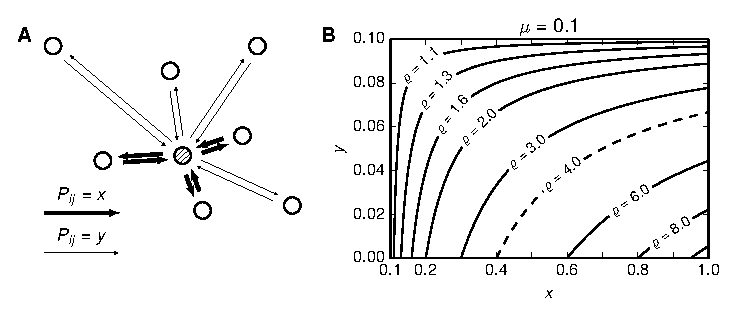
\includegraphics[width=0.9\linewidth]{two_point_full_figure.pdf}
\captionof{figure}{\color{Green} Figure caption}
\end{center}\vspace{1cm}

In hac habitasse platea dictumst. Etiam placerat, risus ac.

Adipiscing lectus in magna blandit:

\begin{center}\vspace{1cm}
\begin{tabular}{l l l l}
\toprule
\textbf{Treatments} & \textbf{Response 1} & \textbf{Response 2} \\
\midrule
Treatment 1 & 0.0003262 & 0.562 \\
Treatment 2 & 0.0015681 & 0.910 \\
Treatment 3 & 0.0009271 & 0.296 \\
\bottomrule
\end{tabular}
\captionof{table}{\color{Green} Table caption}
\end{center}\vspace{1cm}

Vivamus sed nibh ac metus tristique tristique a vitae ante. Sed lobortis mi ut arcu fringilla et adipiscing ligula rutrum. Aenean turpis velit, placerat eget tincidunt nec, ornare in nisl. In placerat.

\begin{center}\vspace{1cm}
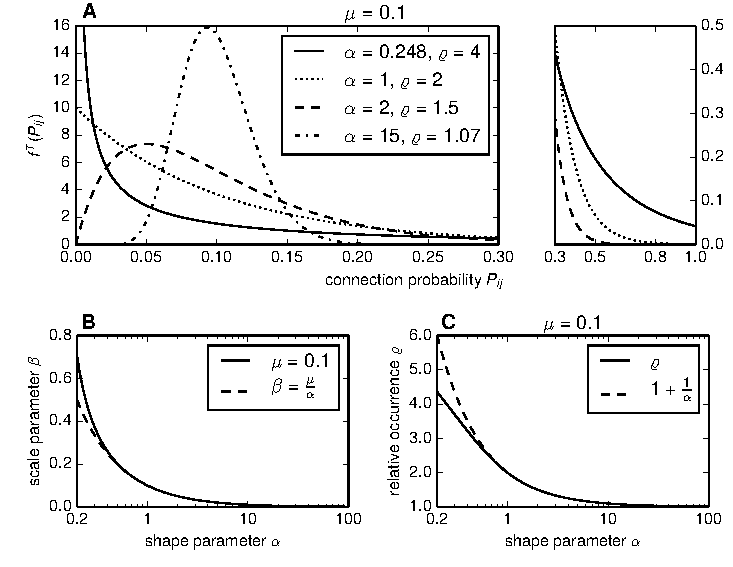
\includegraphics[width=0.9\linewidth]{gamma_figure.pdf}
\captionof{figure}{\color{Green} Figure caption}
\end{center}\vspace{1cm}

%-----------------------------------------------------------------------------
%	CONCLUSIONS
%-----------------------------------------------------------------------------

\section*{Conclusions}

\begin{itemize}
\item Pellentesque eget orci eros. Fusce ultricies, tellus et pellentesque fringilla, ante massa luctus libero, quis tristique purus urna nec nibh. Phasellus fermentum rutrum elementum. Nam quis justo lectus.
\item Vestibulum sem ante, hendrerit a gravida ac, blandit quis magna.
\item Donec sem metus, facilisis at condimentum eget, vehicula ut massa. Morbi consequat, diam sed convallis tincidunt, arcu nunc.
\item Nunc at convallis urna. isus ante. Pellentesque condimentum dui. Etiam sagittis purus non tellus tempor volutpat. Donec et dui non massa tristique adipiscing.
\end{itemize}


%-----------------------------------------------------------------------------
%	FORTHCOMING RESEARCH
%-----------------------------------------------------------------------------

\section*{Forthcoming Research}

Vivamus molestie, risus tempor vehicula mattis, libero arcu volutpat purus, sed blandit sem nibh eget turpis. Maecenas rutrum dui blandit lorem vulputate gravida. Praesent venenatis mi vel lorem tempor at varius diam sagittis. Nam eu leo id turpis interdum luctus a sed augue. Nam tellus.

 %----------------------------------------------------------------------------
%	REFERENCES
%-----------------------------------------------------------------------------

\nocite{*} % Print all references regardless of whether they were cited in the poster or not
\bibliographystyle{plain} % Plain referencing style
\bibliography{sample} % Use the example bibliography file sample.bib

%-----------------------------------------------------------------------------
%	ACKNOWLEDGEMENTS
%-----------------------------------------------------------------------------

\section*{Acknowledgements}

Etiam fermentum, arcu ut gravida fringilla, dolor arcu laoreet justo, ut imperdiet urna arcu a arcu. Donec nec ante a dui tempus consectetur. Cras nisi turpis, dapibus sit amet mattis sed, laoreet.

%-----------------------------------------------------------------------------


  
  \printbibliography  

\end{multicols}

%% \begin{columns}
%%   %
%%   \begin{column}{.5\textwidth}
%%     
\begin{abstract}
  \medskip
  
  Overrepresentation of bidirectional connections in local cortical networks has been repeatedly reported and is in the focus of the ongoing discussion of non-random connectivity.
  %
  Here we show in a brief mathematical analysis that in a network in which connection probabilities are symmetric in pairs, $P_{ij} = P_{ji}$, the occurrence of bidirectional connections and non-random structures are inherently linked; an overabundance of reciprocally connected pairs emerges necessarily when the network structure deviates from a random network in any form.
  %
  %For two distributions of connection probabilities, the discrete two-point distribution and continuous gamma distribution, we quantify how a more organized structure increases reciprocity in the network.

\end{abstract}
  
%% \section*{Introduction}

Increasing evidence implies that \textbf{cortical microcircuitry is highly structured} \cite{Song2005,Perin2011}.
%
The relative occurrence of bidirectionally connected pairs has been of particular interest: 


%%   \end{column}
%%   %
%%   \begin{column}{.5\textwidth}

%%       
\section*{Results}

\textit{Define a random network model in which node-to-node connection probabilities themselves follow a random distribution; some pairs of neurons have a higher chance to be connected than others.}


Consider a random network model of $N$ neurons in which a connection from node $i$ to node $j$ exists with probability $P_{ij}$.
%
Here, the $P_{ij}$, with $i,j = 1,\dots,N$ and $i \neq j$, are identically distributed random variables in $[0,1]$, yielding a probability of connection for each ordered pair of nodes in the network.


\textit{Next, calculate the overrepresentation of bidirectional connection as we would measure in an experiment.}

The overall connection probability $\mu$, that is the chance to have a connection from a random node $i$ to another node $j$, is
\begin{align}
\mu = \E(P_{ij}).
\end{align}
For example, if the $P_{ij}$ have a probability density function $f$ with essential support in $[0,1]$, we can compute the connection fraction as
\begin{align}
  \mu = \int_0^1 x f(x)\,dx.
\end{align}
The probability for random pair of nodes $i$ and $j$ to be connected reciprocally is then
\begin{align}
P_{\mathrm{rec}} = \E(P_{ij} P_{ji}).
\end{align}



%%   \end{column}
%% \end{columns}


\end{document}
